\documentclass[11pt]{beamer}

\usepackage{unicode-math}
\usepackage{amsmath}
\usepackage{amsfonts}
\usepackage{amssymb}
\usepackage[style=ddmmyyyy]{datetime2}
\usepackage{graphicx}
\usepackage{hyperref}
\usepackage{fontspec}
\usepackage{relsize}
\usepackage{xparse}
\usepackage{leftindex}
\usepackage[table]{xcolor}

\makeatletter
\def\input@path{{../../theme/}}
\makeatother

\usetheme[subsectionpage=progressbar]{mis}

\setsansfont{Lato}[Numbers=OldStyle]
\setmathfont{Asana Math}[Scale=MatchLowercase, Style=Alternate]
\setmonofont{Consolas}[Scale=MatchLowercase]

\title{Đại số quan hệ}
\institute{Khoa Hệ thống thông tin quản lý}
\author{Lê Thành Văn}
\date{\today}
% package setting
\hypersetup {
	colorlinks = true
}
%\usecolortheme{seahorse}
% graphic path
\graphicspath{{../../media/}}

%
\AtBeginSection{
  \frame{
    \sectionpage
  }
}
%newcommand
\newcommand{\mmm}[1]{\mathlarger{\mathlarger{\mathlarger#1}}}%
\newcommand{\ppi}[2]{\mmm{\pi}_{#1}\left(#2\right)}%
\newcommand{\psig}[2]{\mmm{\sigma}_{#1}\left(#2\right)}%
\newcommand{\prho}[2]{\mmm{\rho}_{#1}\left(#2\right)}%
\NewDocumentCommand{\join}{o}{%
  \IfNoValueTF{#1}{
    ~\mathlarger\bowtie~
  }{
    ~\mathlarger\bowtie_{#1}~
  }%
}%
\DeclareMathSymbol{\mhyphen}{\mathord}{AMSa}{"39}

\begin{document}
  \begin{frame}
    \titlepage
  \end{frame}
  \section{Giới thiệu}
  \subsection{Đại số quan hệ}
  \begin{frame}
    \textbf{Đại số quan hệ} là ngôn ngữ hình thức cho mô hình quan hệ được phát triển trước SQL. 
    Đại số quan hệ còn có thể được hiểu là tập các thao tác trên mô hình quan hệ, được sử dụng như là cơ sở cho việc cài đặt và tối ưu các câu lệnh truy vấn.
  \end{frame}
  \begin{frame}
    Một số khái niệm của đại số quan hệ được tích hợp vào các câu lệnh truy vấn của SQL, 
    do đó việc tìm hiểu về đại số quan hệ là bệ phóng để xây dựng và thực thi các câu lệnh SQL một cách có hiệu quả.
  \end{frame}
  \subsection{Các khái niệm chung}
  \begin{frame}
    \uncover<1->{Như tên gọi, các đối tượng chính trong đại số quan hệ gồm:}
    \begin{itemize}
      \item<2-> Các quan hệ.
      \item<3-> Những thao tác trên quan hệ.
    \end{itemize}  
  \end{frame}
  \begin{frame}
    Những thao tác thường được xét đến bao gồm
    \begin{itemize}
      \item Thao tác trên một quan hệ: phép chọn, phép chiếu.
      \item Thao tác trên nhiều quan hệ: phép hợp, phép giao, phép trừ, phép kết.
    \end{itemize}
    Ta gọi những thao tác này là các toán tử.
  \end{frame}
  \begin{frame}
    Sự kết hợp giữa các quan hệ cùng với các thao tác theo đúng cấu trúc được gọi là biểu thức quan hệ. \\
    \textit{Ví dụ}. $\ppi{A = 1}{R \times S}$ (chọn ra những dòng có cột $A$ bằng 1 từ 
    tích Đề-các của $R$ và $S$).
  \end{frame}
  \begin{frame}
    Kết quả của một biểu thức quan hệ là một quan hệ.
  \end{frame}
  \section{Các toán tử cơ bản}
  \subsection{Các ký hiệu cơ bản}
  \begin{frame}
    Để tiện cho việc theo dõi, chúng ta quy ước ký hiệu như sau:
    \begin{itemize}
      \item Tên quan hệ được viết in hoa toàn bộ: $R$, $S$, $CUSTOMER$, \dots 
      \item Tên cột được viết dính liền và viết in hoa chữ cái đầu mỗi từ: Age, CustomerId, \dots
      \item Cột $X$ của quan hệ $R$ sẽ được ký hiệu $R.X$ hoặc $R[X]$.
      \item Một dòng trong quan hệ $\{\langle t_1, t_2, \dots, t_n\rangle\}$
    \end{itemize}
  \end{frame}
  \subsection{Các phép toán tập hợp}
  \begin{frame}
    \uncover<1->{Đại số quan hệ được xây dựng trên lý thuyết tập hợp, nên ta có một số toán tử sau:}
    \begin{itemize}
      \item<2-> Phép hợp $R \cup S$.
      \item<2-> Phép giao $R \cap S$.
      \item<2-> Phép trừ $R \setminus S$ hoặc $R - S$.
      \item<2-> Phép tích Đề-các $R \times S$.
    \end{itemize}
  \end{frame}
  \begin{frame}
    Trong đó, phép hợp, phép giao và phép trừ yêu cầu hai quan hệ $R$ và $S$ phải khả hợp.
  \end{frame}
  \begin{frame}
    \uncover<1->{\textit{Định nghĩa}. Hai quan hệ $R(A_0, A_1, \dots, A_n)$ và $S(B_0, B_1, \dots, B_m)$ được gọi là khả hợp khi:}
    \begin{itemize}
      \item<2-> Có cùng số cột, $n = m$.
      \item<3-> Miền xác định của $A_i$ phải giống miền xác định của $B_i$, $i = 0, 1, \dots, n$.
    \end{itemize}
  \end{frame}
  \begin{frame}
    \textit{Ví dụ}. Hai quan hệ sau đây là khả hợp:
    \begin{center}
      \begin{columns}[T]
        \begin{column}{0.5\textwidth}
          \begin{tabular}{|l|l|}
            \hline
            Tên & NgàySinh \\ \hline
            Tùng & 12/08/1955 \\ \hline
            Hằng & 19/07/1968 \\ \hline        
          \end{tabular}
        \end{column}
        \begin{column}{0.5\textwidth}
          \begin{tabular}{|l|l|}
            \hline
            Tên & SinhNhật \\ \hline
            Trinh & 05/07/1985 \\ \hline
            Khang & 29/02/1980 \\ \hline 
            Minh & 30/12/1988 \\ \hline
          \end{tabular}
        \end{column}
      \end{columns}
    \end{center}
  \end{frame}
  \begin{frame}{Quy ước}
    Kết quả của $R \cup S$, $R \cap S$ và $R \setminus S$ là một quan hệ với tên cột là tên cột của $R$.
  \end{frame}
  \begin{frame}{Phép hợp}
    \textit{Định nghĩa}. Kết quả của phép hợp $R \cup S$ là tập hợp những dòng có trong $R$ \textbf{hoặc} có trong $S$.
    $$R \cup S = \{u\ |\ u \in R \vee u \in S\}$$
  \end{frame}
  \begin{frame}
    \begin{columns}[T]
      \begin{column}{0.3\textwidth}
        \centering $R$
        \medskip \\
        \begin{tabular}{|c|c|}
          \hline
          $\textbf{A}_0$ & $\textbf{A}_1$ \\[0.5ex] \hline\hline
          $\alpha$ & 1 \\ \hline
          $\alpha$ & 2 \\ \hline
          $\beta$ & 1 \\ \hline
        \end{tabular}
      \end{column}
      \begin{column}{0.3\textwidth}
        \centering $S$
        \medskip \\
        \begin{tabular}{|c|c|}
          \hline
          $\textbf{B}_0$ & $\textbf{B}_1$ \\[0.5ex] \hline\hline
          $\alpha$ & 2 \\ \hline
          $\beta$ & 3 \\ \hline
        \end{tabular}
      \end{column}
      \begin{column}{0.3\textwidth}
        \centering $R \cup S$
        \medskip \\
        \begin{tabular}{|c|c|}
          \hline
          $\textbf{A}_0$ & $\textbf{A}_1$ \\[0.5ex] \hline\hline
          $\alpha$ & 1 \\ \hline
          $\alpha$ & 2 \\ \hline
          $\beta$ & 1 \\ \hline
          $\beta$ & 3 \\ \hline
        \end{tabular}
      \end{column}
    \end{columns}
  \end{frame}
  \begin{frame}{Phép giao}
    \textit{Định nghĩa}. Kết quả của phép giao $R \cap  S$ là tập hợp những dòng có trong $R$ \textbf{và} có trong $S$.
    $$R \cap S = \{u\ |\ u \in R \wedge u \in S\}$$
  \end{frame}
  \begin{frame}
    \begin{columns}[T]
      \begin{column}{0.3\textwidth}
        \centering $R$
        \medskip \\
        \begin{tabular}{|c|c|}
          \hline
          $\textbf{A}_0$ & $\textbf{A}_1$ \\[0.5ex] \hline\hline
          $\alpha$ & 1 \\ \hline
          $\alpha$ & 2 \\ \hline
          $\beta$ & 1 \\ \hline
        \end{tabular}
      \end{column}
      \begin{column}{0.3\textwidth}
        \centering $S$
        \medskip \\
        \begin{tabular}{|c|c|}
          \hline
          $\textbf{B}_0$ & $\textbf{B}_1$ \\[0.5ex] \hline\hline
          $\alpha$ & 2 \\ \hline
          $\beta$ & 3 \\ \hline
        \end{tabular}
      \end{column}
      \begin{column}{0.3\textwidth}
        \centering $R \cap S$
        \medskip \\
        \begin{tabular}{|c|c|}
          \hline
          $\textbf{A}_0$ & $\textbf{A}_1$ \\[0.5ex] \hline\hline
          $\alpha$ & 2 \\ \hline
        \end{tabular}
      \end{column}
    \end{columns}
  \end{frame}
  \begin{frame}{Phép trừ}
    \textit{Định nghĩa}. Kết quả của phép trừ $R \setminus S$ là tập hợp những dòng \textbf{có} trong $R$ 
    \textbf{nhưng không có} trong $S$.
    $$R \setminus S = \{u\ |\ u \in R \wedge u \not\in S\}$$
  \end{frame}
  \begin{frame}
    \begin{columns}[T]
      \begin{column}{0.3\textwidth}
        \centering $R$
        \medskip \\
        \begin{tabular}{|c|c|}
          \hline
          $\textbf{A}_0$ & $\textbf{A}_1$ \\[0.5ex] \hline\hline
          $\alpha$ & 1 \\ \hline
          $\alpha$ & 2 \\ \hline
          $\beta$ & 1 \\ \hline
        \end{tabular}
      \end{column}
      \begin{column}{0.3\textwidth}
        \centering $S$
        \medskip \\
        \begin{tabular}{|c|c|}
          \hline
          $\textbf{B}_0$ & $\textbf{B}_1$ \\[0.5ex] \hline\hline
          $\alpha$ & 2 \\ \hline
          $\beta$ & 3 \\ \hline
        \end{tabular}
      \end{column}
      \begin{column}{0.3\textwidth}
        \centering $R \setminus S$
        \medskip \\
        \begin{tabular}{|c|c|}
          \hline
          $\textbf{A}_0$ & $\textbf{A}_1$ \\[0.5ex] \hline\hline
          $\alpha$ & 1 \\ \hline
          $\beta$ & 1 \\ \hline
        \end{tabular}
      \end{column}
    \end{columns}
  \end{frame}
  \begin{frame}{Phép tích Đề-các}
    \textit{Định nghĩa}. Cho quan hệ $R$ có $m$ cột và quan hệ $S$ có $n$ cột, 
    kết quả của phép tích Đề-các $R \times S$ là tập hợp những dòng có $m + n$ cột, 
    trong đó $m$ cột đầu là một dòng của $R$ và $n$ cột sau là một dòng của $S$.
    $$R \times S = \{\langle u, v\rangle \ |\ u \in R \wedge v \in S\}$$
  \end{frame}
  \begin{frame}
    \begin{columns}[T]
      \begin{column}{0.25\textwidth}
        \centering $R$
        \medskip \\
        \begin{tabular}{|c|c|}
          \hline
          $\textbf{A}_0$ & $\textbf{A}_1$ \\[0.5ex] \hline\hline
          $\alpha$ & 1 \\ \hline
          $\alpha$ & 2 \\ \hline
          $\beta$ & 1 \\ \hline
        \end{tabular}
      \end{column}
      \begin{column}{0.25\textwidth}
        \centering $S$
        \medskip \\
        \begin{tabular}{|c|c|}
          \hline
          $\textbf{B}_0$ & $\textbf{B}_1$ \\[0.5ex] \hline\hline
          $\gamma$ & 2 \\ \hline
          $\delta$ & 3 \\ \hline
        \end{tabular}
      \end{column}
      \begin{column}{0.4\textwidth}
        \centering $R \times S$
        \medskip \\
        \begin{tabular}{|c|c|c|c|}
          \hline
          $\textbf{A}_0$ & $\textbf{A}_1$ & $\textbf{B}_0$ & $\textbf{B}_1$\\[0.5ex] \hline\hline
          $\alpha$ & 1 & $\gamma$ & 2 \\ \hline
          $\alpha$ & 2 & $\gamma$ & 2 \\ \hline
          $\beta$ & 1 & $\gamma$ & 2 \\ \hline
          $\alpha$ & 1 & $\delta$ & 3 \\ \hline
          $\alpha$ & 2 & $\delta$ & 3\\ \hline
          $\beta$ & 1 & $\delta$ & 3\\ \hline
        \end{tabular}
      \end{column}
    \end{columns}
  \end{frame}
  \begin{frame}{Tính chất}
    \uncover<1->{
      Tính giao hoán
      \begin{itemize}
        \item $R \cup S = S \cup R$.
        \item $R \cap S = S \cap R$.
      \end{itemize}
    }
    \uncover<2->{
      Tính kết hợp
      \begin{itemize}
        \item $R \cup (S \cup T) = (R \cup S) \cup T$.
        \item $R \cap (S \cap T) = (R \cap S) \cap T$.
      \end{itemize}
    }
    \uncover<3->{
      Tính phân phối
      \begin{itemize}
        \item $R \cup (S \cap T) = (R \cup S) \cap (R \cup T)$.
        \item $R \cap (S \cup T) = (R \cap S) \cup (R \cap T)$.
      \end{itemize}
    }
  \end{frame}
  \begin{frame}{Tính chất (tiếp)}
    Phép tích Đề-các không có tính giao hoán
    $$R \times S \neq S \times R$$
  \end{frame}
  \begin{frame}{Tính chất (tiếp)}
    Phép tích Đề-các có tính phân phối đối với phép hợp, phép giao và phép trừ
    \begin{gather*}
      R \times (S \cup P) = (R \times S) \cup (R \times P) \\
      R \times (S \cap P) = (R \times S) \cap (R \times P) \\
      R \times (S \setminus P) = (R \times S) \setminus (R \times P)
    \end{gather*}
  \end{frame}
  \subsection{Các toán tử quan hệ}
  \begin{frame}{Phép chiếu}
    \textit{Định nghĩa}. Cho quan hệ $R$ và một tập hợp $X$ gồm các cột có trong $R$, 
    kết quả của phép chiếu $\ppi{X}{R}$ là một quan hệ chỉ bao gồm những cột có trong $X$.
    Nói cách khác, ta loại bỏ khỏi $R$ những cột không có trong $X$. 
  \end{frame}
  \begin{frame}
    \begin{columns}[T]
      \begin{column}{0.4\textwidth}
        \centering $R$
        \bigskip \\
        \begin{tabular}{|c|c|c|}
          \hline
          \textbf{A} & \textbf{B} & \textbf{C}  \\[0.5ex] \hline\hline
          $\alpha$ & 1 & a\\ \hline
          $\alpha$ & 2 & a\\ \hline
          $\beta$ & 1 & b\\ \hline
        \end{tabular}
      \end{column}
      \begin{column}{0.25\textwidth}
        \centering $\ppi{\text{A, B}}{R}$
        \medskip \\
        \begin{tabular}{|c|c|}
          \hline
          \textbf{A} & \textbf{B} \\[0.5ex] \hline\hline
          $\alpha$ & 1\\ \hline
          $\alpha$ & 2\\ \hline
          $\beta$ & 1\\ \hline
        \end{tabular}
      \end{column}
      \begin{column}{0.25\textwidth}
        \centering $\ppi{\text{A, C}}{R}$
        \medskip \\
        \begin{tabular}{|c|c|}
          \hline
          \textbf{A} & \textbf{C} \\[0.5ex] \hline\hline
          $\alpha$ & a\\ \hline
          $\beta$ & b\\ \hline
        \end{tabular}
      \end{column}
    \end{columns}
  \end{frame}
  \begin{frame}{Tính chất phép chiếu}
    Phép chiếu có tính lũy đẳng, nghĩa là
    $$\ppi{X}{\ppi{X}{R}} = \ppi{X}{R}$$
  \end{frame}
  \begin{frame}{Tính chất phép chiếu (tiếp)}
    Ngoài ra, một chuỗi các \textit{phép chiếu hợp lệ} có cùng kết quả với phép chiếu ngoài cùng
    $$\ppi{Y}{\ppi{X}{R}} = \ppi{Y}{R}$$
    Phép chiếu hợp lệ là phép chiếu chỉ lấy ra những cột đang có trong quan hệ.
  \end{frame}
  \begin{frame}{Tính chất phép chiếu (tiếp)}
    Phép chiếu có tính phân phối đối với phép hợp, nghĩa là
    $$\ppi{X}{R \cup S} = \ppi{X}{R} \cup \ppi{X}{S}$$
    Tuy nhiên, phép chiếu lại không có tính phân phối với phép giao và phép trừ.
  \end{frame}
  \begin{frame}{Phép chọn}
  \textit{Định nghĩa}. Cho quan hệ $R$ và điều kiện so sánh $\theta$, kết quả của 
  phép chọn $\psig{\theta}{R}$ là một quan hệ gồm \textbf{các dòng} mà điều kiện $\theta$ là đúng.
  \end{frame}
  \begin{frame}{Điều kiện so sánh}
    \uncover<1->{Điều kiện so sánh gồm ba dạng:}
    \begin{itemize}
      \item<2-> $\langle\text{tên cột 1}\rangle\langle\text{phép so sánh}\rangle\langle\text{tên cột 2}\rangle$.
      \item<3-> $\langle\text{tên cột}\rangle\langle\text{phép so sánh}\rangle\langle\text{giá trị vô hướng}\rangle$.
      \item<4-> $\langle\text{tên cột}\rangle~\text{có (không) phải trống?}$
    \end{itemize}
  \end{frame}
  \begin{frame}
    \uncover<1->{Trong đó:}
    \begin{itemize}
      \item<2-> $\langle\text{phép so sánh}\rangle$ là các phép $<, >, \leq, \geq, =, \neq$.
      \item<3-> $\langle\text{giá trị vô hướng}\rangle$ là một giá trị thuộc về miền xác định của $\langle\text{tên cột}\rangle$.
    \end{itemize}
  \end{frame}
  \begin{frame}
    \uncover<1->{Ngoài ra, còn có thể kết hợp nhiều điều kiện so sánh với nhau 
    bằng $\wedge$ (phép hội), $\vee$ (phép tuyển) và $\neg$ (phép phủ định).}
    \begin{itemize}
      \item<2-> $\varphi \wedge \psi$: cả hai điều kiện được thỏa.
      \item<3-> $\varphi \vee \psi$: một trong hai điều kiện được thỏa.
      \item<4-> $\neg \varphi$: phủ định điều kiện $\varphi$ (ví dụ: $\neg (A < 5) \Leftrightarrow A \geq 5$).
    \end{itemize}
  \end{frame}
  \begin{frame}
    \begin{columns}[T]
      \begin{column}{0.3\textwidth}
        \centering $R$
        \bigskip \\
        \begin{tabular}{|c|c|c|}
          \hline
          \textbf{A} & \textbf{B} & \textbf{C}  \\[0.5ex] \hline\hline
          $\alpha$ & 1 & a\\ \hline
          $\alpha$ & 2 & a\\ \hline
          $\beta$ & 1 & b\\ \hline
        \end{tabular}
      \end{column}
      \begin{column}{0.3\textwidth}
        \centering $\psig{\text{A} = \alpha}{R}$
        \medskip \\
        \begin{tabular}{|c|c|c|}
          \hline
          \textbf{A} & \textbf{B} & \textbf{C} \\[0.5ex] \hline\hline
          $\alpha$ & 1 & a\\ \hline
          $\alpha$ & 2 & a\\ \hline
        \end{tabular}
      \end{column}
      \begin{column}{0.3\textwidth}
        \centering $\psig{\text{A} = \alpha \vee \text{B} < 2}{R}$
        \medskip \\
        \begin{tabular}{|c|c|c|}
          \hline
          \textbf{A} & \textbf{B} & \textbf{C} \\[0.5ex] \hline\hline
          $\alpha$ & 1 & a\\ \hline
          $\beta$ & 1 & b\\ \hline
        \end{tabular}
      \end{column}
    \end{columns}
  \end{frame}
  \begin{frame}{Tính chất phép chọn}
    \uncover<1->{Cho quan hệ $R$, hai điều kiện so sánh $\varphi$ và $\psi$, ta có các tính chất sau:}
    \begin{itemize}
      \item<2-> $\psig{\varphi}{\psig{\psi}{R}} = \psig{\varphi \wedge \psi}{R} = \psig{\varphi}{R} \cap \psig{\psi}{R}$
      \item<3-> $\psig{\varphi \vee \psi}{R} = \psig{\varphi}{R} \cup \psig{\psi}{R}$
      \item<4-> $\psig{\neg \varphi}{R} = R \setminus \psig{\varphi}{R}$
    \end{itemize}
  \end{frame}
  \begin{frame}{Tính chất phép chọn (tiếp)}
    Phép chọn có tính phân phối đối với phép hợp, phép giao và phép trừ.
    \begin{itemize}
      \item $\psig{\theta}{R \cup S} = \psig{\theta}{R} \cup \psig{\theta}{S}$
      \item $\psig{\theta}{R \cup S} = \psig{\theta}{R} \cup \psig{\theta}{S}$
      \item $\psig{\theta}{R \setminus S} = \psig{\theta}{R} \setminus \psig{\theta}{S}$
    \end{itemize}
  \end{frame}
  \begin{frame}
    \textit{Lưu ý}. Về cơ bản, giữa phép chọn và phép chiếu \textbf{không có tính giao hoán}, nghĩa là
    $$
    \ppi{X}{\psig{\theta}{R}} \neq \psig{\theta}{\ppi{X}{R}}
    $$
    Dấu bằng chỉ xảy ra nếu như các cột trong điều kiện so sánh $\theta$ là một tập con 
    của các cột chiếu $X$.
  \end{frame}
  \begin{frame}{Phép gán}
    \uncover<1->{Để tiện cho việc theo dõi, người ta thường tách một biểu thức quan hệ ra thành nhiều bước ngắn,
    vì thế, cần đặt một tên tạm cho kết quả ở mỗi bước.} \\
    \uncover<2->{Phép gán được ký hiệu bằng $\leftarrow$}.
  \end{frame}
  \begin{frame}
    \uncover<1->{Chẳng hạn, biểu thức $\ppi{X}{\psig{\theta}{R}}$ có thể được ghi thành:}
    \begin{enumerate}
      \item<2-> $T \leftarrow \psig{\theta}{R}$.
      \item<3-> $\ppi{X}{T}$.
    \end{enumerate}
  \end{frame}
  \begin{frame}{Phép đổi tên}
    \textit{Định nghĩa}. Cho quan hệ $R$ và cách đổi tên $N$, kết quả của phép đổi tên
    $\prho{N}{R}$ vẫn là những thông tin đó, nhưng với tên quan hệ và tên cột được thay đổi dựa theo cách đổi tên $N$.
  \end{frame}
  \begin{frame}{Cách đổi tên}
    \uncover<1->{Cách đổi tên $N$ có ba dạng sau:}
    \begin{itemize}
      \item<2-> $A/B$: đổi tên cột $B$ thành $A$.
      \item<3-> $(B_0, B_1, \dots, B_n)$: đổi tên cột đầu tiên thành $B_0$, cột thứ hai thành $B_1$, \dots
      \item<4-> $S(B_0, B_1, \dots, B_n)$: đổi tên quan hệ thành $S$, đổi tên cột đầu tiên thành $B_0$, cột thứ hai thành $B_1$, \dots
    \end{itemize}
  \end{frame}
  \begin{frame}
    \uncover<1->{Cho quan hệ $R(A, B, C)$, khi đó:}
    \uncover<2->{
      \begin{itemize}
        \item $\prho{D/A}{R} = R(D, B, C)$.
        \item $\prho{(D, E)}{R} = R(D, E, C)$.
        \item $\prho{S(D, E, F)}{R} = S(D, E, F)$.
      \end{itemize}
    }
  \end{frame}
  \begin{frame}
    Phép đổi tên thường được dùng trong trường hợp sử dụng đến phép kết 
    hoặc có tính toán giữa các cột với nhau.
  \end{frame}
  \section{Các toán tử nâng cao}
  \subsection{Phép kết}
  \begin{frame}{Phép kết theta}
    \textit{Định nghĩa}. Cho hai quan hệ $R$ và $S$, điều kiện so sánh $\theta$, kết quả của phép kết theta
    $R \join[\theta] S$ là một quan hệ gồm những dòng thỏa mãn $\theta$ được chọn ra từ tích Đề-các $R \times S$.
    Nói cách khác,
    $$
    R \join[\theta] S = \psig{\theta}{R \times S}
    $$
  \end{frame}
  \begin{frame}
    Do phép kết dùng để kết nối hai quan hệ với nhau, nên điều kiện so sánh thường là
    $$\langle\text{tên cột bảng 1}\rangle\langle\text{phép so sánh}\rangle\langle\text{tên cột bảng 2}\rangle$$
  \end{frame}
  \begin{frame}
    \begin{columns}[T]
      \begin{column}{0.3\textwidth}
        \centering $R$
        \bigskip \\
        \begin{tabular}{|c|c|c|}
          \hline
          \textbf{A} & \textbf{B} & \textbf{C}  \\[0.5ex] \hline\hline
          \bullet & 2 & \bullet\\ \hline
          \bullet & 5 & \bullet\\ \hline
          \bullet & 8 & \bullet\\ \hline
        \end{tabular}
      \end{column}
      \begin{column}{0.2\textwidth}
        \centering $S$
        \bigskip \\
        \begin{tabular}{|c|c|}
          \hline
          \textbf{D} & \textbf{E} \\[0.5ex] \hline\hline
          3 & \bullet\\ \hline
          6 & \bullet\\ \hline
        \end{tabular}
      \end{column}
      \begin{column}{0.5\textwidth}
        \centering $R \join[B < D] S$
        \medskip \\
        \begin{tabular}{|c|c|c|c|c|}
          \hline
          \textbf{A} & \textbf{B} & \textbf{C} & \textbf{D} & \textbf{E}\\[0.5ex] \hline\hline
          \bullet & 2 & \bullet & 3 & \bullet\\ \hline
          \bullet & 2 & \bullet & 6 & \bullet\\ \hline
          \bullet & 5 & \bullet & 6 & \bullet\\ \hline
        \end{tabular}
      \end{column}
    \end{columns}
  \end{frame}
  \begin{frame}{Phép kết bằng}
    \textit{Định nghĩa}. Phép kết bằng là phép kết có điều kiện so sánh là so sánh bằng.
  \end{frame}
  \begin{frame}{Phép kết tự nhiên}
    \textit{Định nghĩa}. Phép kết tự nhiên là phép kết bằng trên những cột cùng tên giữa hai quan hệ.
    Ký hiệu $R \join S$. Ngoài ra, trong kết quả của phép kết tự nhiên, các cột cùng tên giữa hai quan hệ
    chỉ xuất hiện một lần.
  \end{frame}
  \begin{frame}
    Cho hai quan hệ $R(A_1, A_2, \dots,A_n, C_1, C_2, \dots, C_k)$ và $S(B_1, B_2, \dots, B_m, C_1, C_2, \dots, C_k)$,
    khi đó
    $$
    R \join S = \ppi{X}{\psig{R.C_1 = S.C_1,\ \dots,\ R.C_k = S.C_k}{R \times S}}
    $$
    với $X = \{A_1, A_2, \dots,A_n, B_1, B_2, \dots, B_m, C_1, C_2, \dots, C_k\}$
  \end{frame}
  \begin{frame}
    \begin{columns}[T]
      \begin{column}{0.3\textwidth}
        \centering $R$
        \medskip \\
        \begin{tabular}{|c|c|c|}
          \hline
          \textbf{A} & \textbf{B} & \textbf{C}  \\[0.5ex] \hline\hline
          $\alpha$ & 2 & a\\ \hline
          $\beta$ & 5 & a\\ \hline
          $\gamma$ & 8 & e\\ \hline
        \end{tabular}
      \end{column}
      \begin{column}{0.3\textwidth}
        \centering $S$
        \medskip \\
        \begin{tabular}{|c|c|}
          \hline
          \textbf{A} & \textbf{E} \\[0.5ex] \hline\hline
          $\alpha$ & x\\ \hline
          $\lambda$ & y\\ \hline
        \end{tabular}
      \end{column}
      \begin{column}{0.3\textwidth}
        \centering $R \join S$
        \medskip \\
        \begin{tabular}{|c|c|c|c|}
          \hline
          \textbf{A} & \textbf{B} & \textbf{C} & \textbf{E}\\[0.5ex] \hline\hline
          $\alpha$ & 2 & a & x \\ \hline
        \end{tabular}
      \end{column}
    \end{columns}
  \end{frame}
  \begin{frame}{Phép kết nửa}
    \textit{Định nghĩa}. Phép kết nửa trái (phải) là phép kết tự nhiên nhưng kết quả không bao gồm
    những cột của bảng trái (phải). Ký hiệu $R~⋉~S$ (trái), $R~⋊~S$ (phải).
  \end{frame}
  \begin{frame}
    \begin{columns}[T]
      \begin{column}{0.3\textwidth}
        \centering $R$
        \medskip \\
        \begin{tabular}{|c|c|c|}
          \hline
          \textbf{A} & \textbf{B} & \textbf{C}  \\[0.5ex] \hline\hline
          $\alpha$ & 2 & a\\ \hline
          $\beta$ & 5 & a\\ \hline
          $\gamma$ & 8 & e\\ \hline
        \end{tabular}
      \end{column}
      \begin{column}{0.3\textwidth}
        \centering $S$
        \medskip \\
        \begin{tabular}{|c|c|}
          \hline
          \textbf{A} & \textbf{E} \\[0.5ex] \hline\hline
          $\alpha$ & x\\ \hline
          $\lambda$ & y\\ \hline
        \end{tabular}
      \end{column}
      \begin{column}{0.3\textwidth}
        \centering $R~⋉~S$
        \medskip \\
        \begin{tabular}{|c|c|c|}
          \hline
          \textbf{A} & \textbf{B} & \textbf{C}\\[0.5ex] \hline\hline
          $\alpha$ & 2 & a \\ \hline
        \end{tabular}
      \end{column}
    \end{columns}
  \end{frame}
  \begin{frame}{Phép phản kết}
    \textit{Định nghĩa}. Kết quả của phép phản kết $R \rhd S$ là những dòng thuộc $R$ nhưng không tham gia
    vào phép kết nửa trái $R~⋉~S$. Nói cách khác
    $$
    R \rhd S = R - R~⋉~S
    $$
  \end{frame}
  \begin{frame}
    \begin{columns}[T]
      \begin{column}{0.3\textwidth}
        \centering $R$
        \medskip \\
        \begin{tabular}{|c|c|c|}
          \hline
          \textbf{A} & \textbf{B} & \textbf{C}  \\[0.5ex] \hline\hline
          $\alpha$ & 2 & a\\ \hline
          $\beta$ & 5 & a\\ \hline
          $\gamma$ & 8 & e\\ \hline
        \end{tabular}
      \end{column}
      \begin{column}{0.3\textwidth}
        \centering $S$
        \medskip \\
        \begin{tabular}{|c|c|}
          \hline
          \textbf{A} & \textbf{E} \\[0.5ex] \hline\hline
          $\alpha$ & x\\ \hline
          $\lambda$ & y\\ \hline
        \end{tabular}
      \end{column}
      \begin{column}{0.3\textwidth}
        \centering $R \rhd S$
        \medskip \\
        \begin{tabular}{|c|c|c|}
          \hline
          \textbf{A} & \textbf{B} & \textbf{C}\\[0.5ex] \hline\hline
          $\beta$ & 5 & a\\ \hline
          $\gamma$ & 8 & e\\ \hline
        \end{tabular}
      \end{column}
    \end{columns}
  \end{frame}
  \begin{frame}{Phép kết ngoài}
    Có thể thấy phép kết tự nhiên chỉ giữ lại những bộ thỏa điều kiện kết.
    Tuy nhiên, trong nhiều trường hợp, cần giữ lại những thông tin không được kết 
    ở bảng trái hoặc bảng phải hoặc cả hai bảng. \\
    Vì thế, người ta bổ sung thêm ba phép kết:
    \begin{itemize}
      \item Phép kết (ngoài) trái $R~⟕~S$.
      \item Phép kết (ngoài) phải $R~⟖~S$.
      \item Phép kết ngoài đầy đủ $R~⟗~S$
    \end{itemize}
  \end{frame}
  \begin{frame}{Phép kết ngoài trái}
    \textit{Định nghĩa}. Kết quả của phép kết ngoài trái $R~⟕~S$ là một quan hệ bao gồm:
    \begin{itemize}
      \item Tất cả những dòng của phép kết tự nhiên $R \join S$.
      \item Tích Đề-các giữa những dòng của phép phản kết $R \rhd S$ và một dòng trống. 
    \end{itemize}
    $$
    R~⟕~S = (R \join S) \cup \left((R \rhd S) \times \{\langle\omega, \omega, \dots, \omega\rangle\}\right)
    $$
  \end{frame}
  \begin{frame}
    Có thể thấy phép kết ngoài trái $R~⟖~S$ giữ nguyên tất cả các dòng của quan hệ bên trái.
  \end{frame}
  \begin{frame}
    \begin{columns}[T]
      \begin{column}{0.3\textwidth}
        \centering $R$
        \medskip \\
        \begin{tabular}{|c|c|c|}
          \hline
          \textbf{A} & \textbf{B} & \textbf{C}  \\[0.5ex] \hline\hline
          $\alpha$ & 2 & a\\ \hline
          $\beta$ & 5 & a\\ \hline
          $\gamma$ & 8 & e\\ \hline
        \end{tabular}
      \end{column}
      \begin{column}{0.3\textwidth}
        \centering $S$
        \medskip \\
        \begin{tabular}{|c|c|}
          \hline
          \textbf{A} & \textbf{E} \\[0.5ex] \hline\hline
          $\alpha$ & x\\ \hline
          $\lambda$ & y\\ \hline
        \end{tabular}
      \end{column}
      \begin{column}{0.3\textwidth}
        \centering $R~⟕~S$
        \medskip \\
        \begin{tabular}{|c|c|c|c|}
          \hline
          \textbf{A} & \textbf{B} & \textbf{C} & \textbf{E}\\[0.5ex] \hline\hline
          $\alpha$ & 2 & a & x\\ \hline
          $\beta$ & 5 & a & \cellcolor{blue!25}$\omega$ \\ \hline
          $\gamma$ & 8 & e & \cellcolor{blue!25}$\omega$ \\ \hline
        \end{tabular}
      \end{column}
    \end{columns}
  \end{frame}
  \begin{frame}{Phép kết ngoài phải}
    Chúng ta có thể định nghĩa phép kết ngoài phải tương tự như phép kết ngoài trái, 
    và ta có công thức:
    $$R~⟖~S = S~⟕~R$$
  \end{frame}
  \begin{frame}
    \begin{columns}[T]
      \begin{column}{0.3\textwidth}
        \centering $R$
        \medskip \\
        \begin{tabular}{|c|c|c|}
          \hline
          \textbf{A} & \textbf{B} & \textbf{C}  \\[0.5ex] \hline\hline
          $\alpha$ & 2 & a\\ \hline
          $\beta$ & 5 & a\\ \hline
          $\gamma$ & 8 & e\\ \hline
        \end{tabular}
      \end{column}
      \begin{column}{0.3\textwidth}
        \centering $S$
        \medskip \\
        \begin{tabular}{|c|c|}
          \hline
          \textbf{A} & \textbf{E} \\[0.5ex] \hline\hline
          $\alpha$ & x\\ \hline
          $\lambda$ & y\\ \hline
        \end{tabular}
      \end{column}
      \begin{column}{0.3\textwidth}
        \centering $R~⟖~S$
        \medskip \\
        \begin{tabular}{|c|c|c|c|}
          \hline
          \textbf{A} & \textbf{B} & \textbf{C} & \textbf{E}\\[0.5ex] \hline\hline
          $\alpha$ & 2 & a & x\\ \hline
          $\lambda$ & \cellcolor{blue!25}$\omega$ & \cellcolor{blue!25}$\omega$ & y \\ \hline
        \end{tabular}
      \end{column}
    \end{columns}
  \end{frame}
  \begin{frame}{Phép kết ngoài đầy đủ}
    Cuối cùng, phép kết ngoài đầy đủ là phần hợp giữa phép kết ngoài trái và phép kết ngoài phải.
    $$
    R~⟗~S = (R~⟕~S) \cup (R~⟖~S)
    $$
  \end{frame}
  \begin{frame}
    \begin{columns}[T]
      \begin{column}{0.3\textwidth}
        \centering $R$
        \medskip \\
        \begin{tabular}{|c|c|c|}
          \hline
          \textbf{A} & \textbf{B} & \textbf{C}  \\[0.5ex] \hline\hline
          $\alpha$ & 2 & a\\ \hline
          $\beta$ & 5 & a\\ \hline
          $\gamma$ & 8 & e\\ \hline
        \end{tabular}
      \end{column}
      \begin{column}{0.3\textwidth}
        \centering $S$
        \medskip \\
        \begin{tabular}{|c|c|}
          \hline
          \textbf{A} & \textbf{E} \\[0.5ex] \hline\hline
          $\alpha$ & x\\ \hline
          $\lambda$ & y\\ \hline
        \end{tabular}
      \end{column}
      \begin{column}{0.3\textwidth}
        \centering $R~⟗~S$
        \medskip \\
        \begin{tabular}{|c|c|c|c|}
          \hline
          \textbf{A} & \textbf{B} & \textbf{C} & \textbf{E}\\[0.5ex] \hline\hline
          $\alpha$ & 2 & a & x\\ \hline
          $\beta$ & 5 & a & \cellcolor{blue!25}$\omega$ \\ \hline
          $\gamma$ & 8 & e & \cellcolor{blue!25}$\omega$ \\ \hline
          $\lambda$ & \cellcolor{blue!25}$\omega$ & \cellcolor{blue!25}$\omega$ & y \\ \hline
        \end{tabular}
      \end{column}
    \end{columns}
  \end{frame}
  \subsection{Phép chia}
  \begin{frame}{Phép chia}
    \textit{Định nghĩa}. Cho hai quan hệ $R$ và $S$, kết quả của phép chia $R \div S$ là 
    quan hệ $T$ sao cho tất cả các dòng của $T \times S$ (tích Đề-các) đều là dòng của $R$.
  \end{frame}
  \begin{frame}
    Từ định nghĩa trên có thể thấy, để $R$ có thể chia được cho $S$ 
    thì tất cả các cột của $S$ phải là cột của $R$. Khi đó
    $$
    R \div S = \ppi{X \setminus Y}{R} \setminus \ppi{X \setminus Y}{{\ppi{X \setminus Y}{R} \times S} \setminus R}
    $$
    trong đó, $X$, $Y$ lần lượt là tập hợp tất cả cột của $R$, $S$.
  \end{frame}
  \begin{frame}
    \begin{columns}[T]
      \begin{column}{0.3\textwidth}
        \centering $R$
        \medskip \\
        \begin{tabular}{|c|c|c|}
          \hline
          \textbf{A} & \textbf{B} & \textbf{C}\\[0.5ex] \hline\hline
          \rowcolor{blue!25}
          1 & 2 & 2\\ \hline
          \rowcolor{blue!25}
          1 & 2 & 6\\ \hline
          4 & 2 & 2\\ \hline
          4 & 5 & 6\\ \hline
        \end{tabular}
      \end{column}
      \begin{column}{0.2\textwidth}
        \centering $S$
        \medskip \\
        \begin{tabular}{|c|}
          \hline
          \textbf{C} \\[0.5ex] \hline\hline
          2\\ \hline
          6\\ \hline          
        \end{tabular}
      \end{column}
      \begin{column}{0.3\textwidth}
        \centering $R \div S$
        \medskip \\
        \begin{tabular}{|c|c|}
          \hline
          \textbf{A} & \textbf{B} \\[0.5ex] \hline\hline
          1 & 2\\ \hline
        \end{tabular}
      \end{column}
    \end{columns}
  \end{frame}
  \begin{frame}
    Phép chia thường được dùng trả lời cho câu hỏi `Tìm tất cả X đã tham gia tất cả Y?'
  \end{frame}
  \subsection{Phép chiếu mở rộng}
  \begin{frame}
    Người ta còn mở rộng phép chiếu bằng cách cho phép thực hiện tính toán trên cột,
    hoặc giữa các cột với nhau. \textit{Lưu ý}: cần đặt tên cho những cột là kết quả của việc tính toán.
  \end{frame}
  \begin{frame}
    \begin{columns}[T]
      \begin{column}{0.3\textwidth}
        \centering $R$
        \bigskip \\
        \begin{tabular}{|c|c|c|}
          \hline
          \textbf{A} & \textbf{B} & \textbf{C}  \\[0.5ex] \hline\hline
          $\alpha$ & 1 & 1\\ \hline
          $\alpha$ & 2 & 2\\ \hline
          $\beta$ & 1 & 3\\ \hline
        \end{tabular}
      \end{column}
      \begin{column}{0.3\textwidth}
        \centering $\ppi{\text{A, B+10}}{R}$
        \medskip \\
        \begin{tabular}{|c|c|}
          \hline
          \textbf{A} & \textbf{B} \\[0.5ex] \hline\hline
          $\alpha$ & 11\\ \hline
          $\alpha$ & 12\\ \hline
          $\beta$ & 11\\ \hline
        \end{tabular}
      \end{column}
      \begin{column}{0.3\textwidth}
        \centering $\ppi{\text{A, D/(B\times C)}}{R}$
        \medskip \\
        \begin{tabular}{|c|c|}
          \hline
          \textbf{A} & \textbf{D} \\[0.5ex] \hline\hline
          $\alpha$ & 1\\ \hline
          $\alpha$ & 4\\ \hline
          $\beta$ & 3\\ \hline
        \end{tabular}
      \end{column}
    \end{columns}
  \end{frame}
  \subsection{Phép gom nhóm}
  \begin{frame}
    Các toán tử vừa được giới thiệu vẫn chưa đủ để trả lời các câu hỏi thống kê, 
    vì thế, người ta bổ sung vào đại số quan hệ hai khái niệm mới là 
    \textbf{hàm gom nhóm} và \textbf{phép gom nhóm}.
  \end{frame}
  \begin{frame}{Hàm gom nhóm}
    Hàm gom nhóm là những hàm có đầu vào là một tập hợp các giá trị và đầu ra là một giá trị duy nhất.
    Có các hàm gom nhóm cơ bản:
    \begin{itemize}
      \item $\mathrm{sum}$: tính tổng tập hợp.
      \item $\mathrm{count}$: đếm số lượng khác trống.
      \item $\mathrm{avg}$: tính giá trị trung bình.
      \item $\mathrm{max}$: tìm giá trị lớn nhất.
      \item $\mathrm{min}$: tìm giá trị nhỏ nhất.
      \item $\mathrm{count\mhyphen distinct}$: đếm số lượng giá trị khác nhau và khác trống.
    \end{itemize}
  \end{frame}
  \begin{frame}{Phép gom nhóm cơ bản}
    Cho quan hệ $R$, một cột gom nhóm $G$, và một hàm gom nhóm $F$, 
    kết quả của phép gom nhóm $\leftindex_{G}{\mathcal{G}}_{F(A)}(R)$ 
    là một quan hệ có hai cột với:
    \begin{itemize}
      \item Cột thứ nhất là một giá trị riêng biệt của $G$.
      \item Cột thứ hai là kết quả của hàm $F$ với đầu vào là những giá trị cột $A$ 
      tương ứng với giá trị riêng biệt của cột thứ nhất.
    \end{itemize}
  \end{frame}
  \begin{frame}
    \begin{columns}[T]
      \begin{column}{0.4\textwidth}
        \centering $R$
        \bigskip \\
        \begin{tabular}{|c|c|}
          \hline
          $\textbf{A}$ & $\textbf{B}$ \\[0.5ex] \hline\hline
          $\alpha$ & 1 \\ \hline
          $\alpha$ & 2 \\ \hline
          $\beta$ & 1 \\ \hline
        \end{tabular}
      \end{column}
      \begin{column}{0.6\textwidth}
        \centering $\leftindex_{A}{\mathcal{G}}_{\mathrm{count}(B)} (R)$
        \medskip \\
        \begin{tabular}{|c|c|}
          \hline
          $\textbf{A}$ & $\mathrm{count}$ \\[0.5ex] \hline\hline
          $\alpha$ & 2 \\ \hline
          $\beta$ & 1 \\ \hline
        \end{tabular}
      \end{column}
    \end{columns}
  \end{frame}
  \begin{frame}{Phép gom nhóm mở rộng}
    Có thể mở rộng phép gom nhóm cho nhiều cột $G_1$, $G_2$, \dots, $G_n$ và 
    nhiều hàm gom nhóm $F_1$, $F_2$, \dots, $F_m$, ký hiệu
    $$
    \leftindex_{G_1,\ G_2,\ \dots,\ G_n}{\mathcal{G}}_{F_1(A_1),\ F_2(A_2),\ \dots,\ F_m(A_m)} (R)
    $$
  \end{frame}
  \begin{frame}
    \textit{Lưu ý}:
    \begin{itemize}
      \item Các cột $A_1$, $A_2$, \dots, $A_m$ không nhất thiết phải khác nhau.
      \item Cần đặt tên cho $F_1(A_1),\ F_2(A_2),\ \dots,\ F_m(A_m)$.
    \end{itemize} 
  \end{frame}
  \begin{frame}
    \begin{columns}[T]
      \begin{column}{0.4\textwidth}
        \centering $R$
        \bigskip \\
        \begin{tabular}{|c|c|c|}
          \hline
          \textbf{A} & \textbf{B} & \textbf{C} \\[0.5ex] \hline\hline
          $\alpha$ & 1 & 7\\ \hline
          $\alpha$ & 2 & 4\\ \hline
          $\beta$ & 1 & 2\\ \hline
          $\beta$ & 1 & 5\\ \hline
        \end{tabular}
      \end{column}
      \begin{column}{0.6\textwidth}
        \centering $\leftindex_{A,\ B}{\mathcal{G}}_{\mathrm{count}(C),\ \mathrm{sum}(C)} (R)$
        \medskip \\
        \begin{tabular}{|c|c|c|c|}
          \hline
          \textbf{A} & \textbf{B} & $\mathrm{count}$ & $\mathrm{sum}$ \\[0.5ex] \hline\hline
          $\alpha$ & 1 & 1 & 7\\ \hline
          $\alpha$ & 2 & 1 & 4\\ \hline
          $\beta$ & 1 & 2 & 7\\ \hline
        \end{tabular}
      \end{column}
    \end{columns}
  \end{frame}
  \section{Ví dụ}
  \begin{frame}
    Cho cơ sở dữ liệu như hình:
    \begin{figure}
      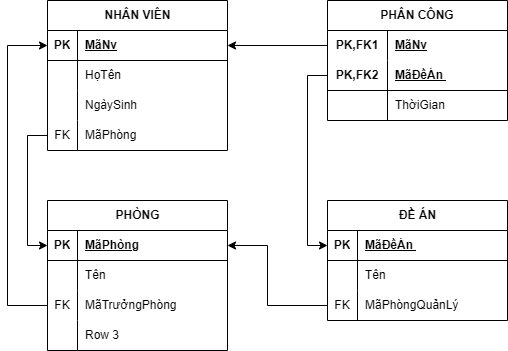
\includegraphics[width=0.9\textwidth]{COS212/schema.png}
    \end{figure}
  \end{frame}
  \begin{frame}
    \uncover<1->{Tìm \textbf{mã nhân viên} không tham gia đề án nào?}
    \begin{enumerate}
      \item<2-> $T \leftarrow \ppi{\text{MãNv}}{\text{NHÂN VIÊN}}$
      \item<3-> $U \leftarrow \ppi{\text{MãNv}}{\text{PHÂN CÔNG}}$      
      \item<4-> $T \setminus U$
    \end{enumerate}
  \end{frame}
  \begin{frame}
    \uncover<1->{Tìm \textbf{mã nhân viên} được phân công tham gia đề án có mã số `TH01' hoặc đề án có mã số `TH02'?}
    \begin{enumerate}
      \item<2-> $T \leftarrow \psig{\text{MãĐềÁn}\ =\ \text{`TH01'} ~\vee~ \text{MãĐềÁn}\ =\ \text{`TH02'}}{\text{PHÂN CÔNG}}$
      \item<3-> $\ppi{\text{MãNv}}{T}$
    \end{enumerate}
  \end{frame}
  \begin{frame}
    \uncover<1->{Tìm \textbf{tên nhân viên} được phân công tham gia đề án có mã số `TH03'?}
    \begin{enumerate}
      \item<2-> $T \leftarrow \psig{\text{MãĐềÁn}\ =\ \text{`TH03'}}{\text{PHÂN CÔNG}}$
      \item<3-> $U \leftarrow \ppi{\text{MãNv}}{T}$
      \item<4-> $\ppi{\text{HọTên}}{U \join \text{NHÂN VIÊN}}$
    \end{enumerate}
  \end{frame}
  \begin{frame}
    \uncover<1->{Tìm \textbf{mã nhân viên} tham gia tất cả các đề án?}
    \begin{enumerate}
      \item<2-> $T \leftarrow \ppi{\text{MãNv, MãĐềÁn}}{\text{PHÂN CÔNG}}$
      \item<3-> $U \leftarrow \ppi{\text{MãĐềÁn}}{\text{ĐỀ ÁN}}$
      \item<4-> $T \div U$
    \end{enumerate}
  \end{frame}
  \begin{frame}
    \uncover<1->{Tìm \textbf{mã đề án} có nhiều nhân viên tham gia nhất?}
    \begin{enumerate}
      \item<2-> $T \leftarrow \leftindex_{\text{MãĐềÁn}}{\mathcal{G}}_{\mathrm{count}(\text{MãNv})}\text{(PHÂN CÔNG)}$
      \item<3-> $\prho{\text{SốLượng}/\mathrm{count}}{T}$
      \item<3-> $U \leftarrow \psig{\text{SốLượng}\ =\ \mathrm{max}\text{(SốLượng)}}{T}$
      \item<4-> $\ppi{\text{MãĐềÁn}}{U}$
    \end{enumerate}
  \end{frame}
\end{document}